\section{Plataforma CA4IoT}
%http://ieeexplore.ieee.org/document/6605518/
%\cite{cite1}http://www.sciencedirect.com/science/article/pii/S0950705116302015
%\cite{cite2}http://ieeexplore.ieee.org/document/6468408/citations?anchor=anchor-paper-citations-ieee&ctx=citations
%\cite{cite3}http://ieeexplore.ieee.org/document/7983223/
%http://ieeexplore.ieee.org/document/6569153/
% Os termos objetos, coisas, objetos inteligentes, dispositivos e n�s s�o utilizados nesse trabalho com o mesmo significado, j� que assim � utilizado na literatura sobre IoT. 

Em XXXxX, Perera descreve o significado de uma arquitetura de sensores em plataformas de IoT, 
n the sensing as a service paradigm, Internet of Things (IoT) Middleware platforms allow data consumers to retrieve the data they want without knowing the underlying technical details of IoT resources (i.e. sen- sors and data processing components). However, configuring an IoT middleware platform and retrieving data is a significant challenge for data consumers as it requires both technical knowledge and domain expertise. In this paper, we propose a knowledge driven approach called Context Aware Sensor Config- uration Model (CASCOM) to simplify the process of configuring IoT middleware platforms, so the data consumers, specifically non-technical personnel, can easily retrieve the data they required. In this pa- per, we demonstrate how IoT resources can be described using semantics in such away that they can later be used to compose service work-flows. Such automated semantic-knowledge-based IoT resource composition approach advances the current research. We demonstrate the feasibility and the usability of our approach through a prototype implementation based on an IoT middleware called Global Sensor Networks (GSN), though our model can be generalized to any other middleware platform. 

\begin{figure}[tbh!]
	\centering
	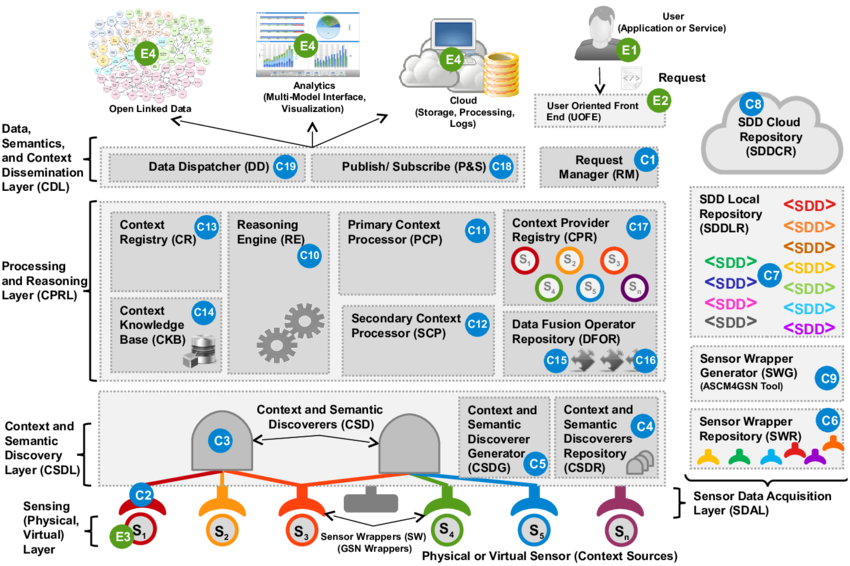
\includegraphics[width=1.0\textwidth]{../images/CA4IOT-component-level-architecture}
	\caption{Arquitetura CA4IOT}
	\label{fig:CA4IOT}
\end{figure}


Em seu trabalho, Pereira identificou os principais pontos necess�rios ao desenvolvimento de um modelo para IoT que viabilize a disponibiliza��o de sensores como servi�os atrav�s da composi��o de m�ltiplos tipos de sensores utilizando diferentes mecanismos de filtros, associa��es e l�gicas. Seu modelo � composto das seguintes funcionalidades principais:

Modelo Aut�nomo:

Baseado no uso (Utility based):

Escal�vel e flex�vel:

F�cil utiliza��o e baixa curva de aprendizado:

